%\subsubsection{TIMELY has no fixed point, is inherently unstable with unpredictable fairness}
We now show that the TIMELY, as described
in Algorithm~\ref{fig:timely_algo} has \emph{no fixed point}. The implication
is that the queue length never converges, nor do the sending rates of the flows.
The system operates in limit cycles, always oscillating. Moreover, while the
system is oscillating, there are \emph{infinite} solutions for the sending rates
of the flows that satisfy the fluid equations at any point. So, even if we can
limit the magnitude of the limit cycles by choosing parameters carefully, we can
make no claims on the fairness of the protocol since the system could be
operating at any of those infinite solutions.

\begin{thm}[No fixed point for TIMELY] 
\label{thm:nofixed}
The system described in Figure~(\ref{fig:timely_model}), has no fixed points.
\end{thm}
\begin{proof}
We prove the result by contradiction. At the fixed point, all
differential equations converge to 0. Thus:
\begin{equation}
\small
{dq}/{dt} = 0 \; \; \mbox{and} \; \;  \sum_{i} R_i(t) =  C
\end{equation} 
Now, either $g_i > 0$ or $g_i  \le 0$. If $g_i \ne 0$, then:
\begin{equation}
\small
\frac{{dg_i}}{{dt}} =  \frac{\alpha }{{\tau_i^*}}( - g_i(t) + \frac{{q(t
                        - \tau ') - q(t - \tau ' - \tau_i^*
                        )}}{{C*{D_{\min RTT}}}})\\
 =   -\frac{\alpha }{{\tau_i^*}} g_i(t)  \ne  0
\end{equation}
Thus, $g_i$ is zero for $dg_i/dt$ to be zero. But then:
\begin{equation}
\small
{dR_i}/{dt} =  {\delta }/{{\tau_i^*}} \ne 0
\end{equation}
Thus, all derivatives cannot be simultaneously 0 and thus the system has no fixed
point.
\end{proof}

If we modify the fluid model very slightly, by moving the equality condition to
the term involving $g_i$, we get:
\begin{equation}
\small
\frac{{dR_i}}{{dt}} = \left\{ \begin{array}{ll}
\frac{\delta }{{\tau_i^*}}, & q(t - \tau ') < C*{T_{low}}\\
\frac{\delta }{{\tau_i^*}}, & g_i < 0\\
 - \frac{{g_i\beta }}{{\tau_i^*}}R(t), & g_i \ge 0\\
 - \frac{\beta }{{\tau_i^*}}(1 - \frac{{C*{T_{high}}}}{{q(t - \tau ')}})R(t), & q(t - \tau ') > C*{T_{high}}
\end{array} \right.\\
\label{eq:timely_r_modified}
\end{equation}

\begin{figure*}[t]
\center
\subfigure[Both flows start at time 0 at 5Gbps] { 
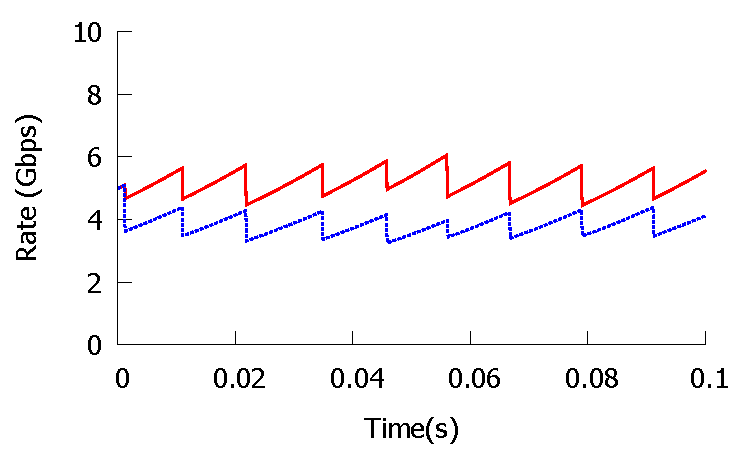
\includegraphics[width=0.3\textwidth]{figures/timely_stability_2f55.pdf}
\label{fig:ts2f55}
}
\subfigure[Both start at 5Gbps, one starts 10ms late] { 
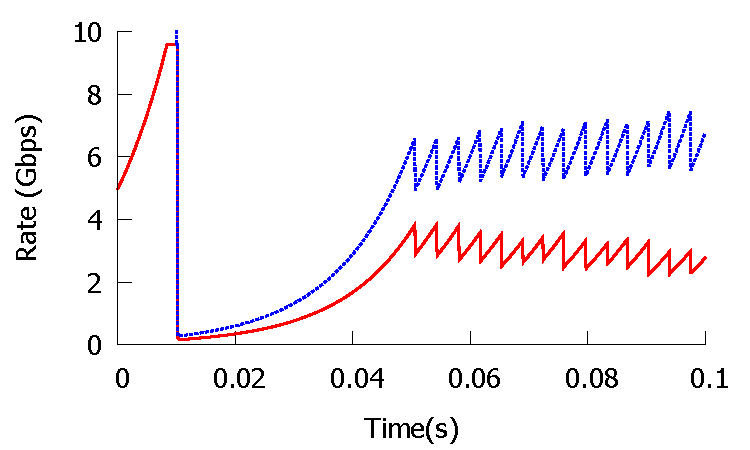
\includegraphics[width=0.3\textwidth]{figures/timely_stability_2ftime.pdf}
\label{fig:ts2f55time}
}
\subfigure[Both start at time 0, one at 7Gbps, other at 3Gbps] { 
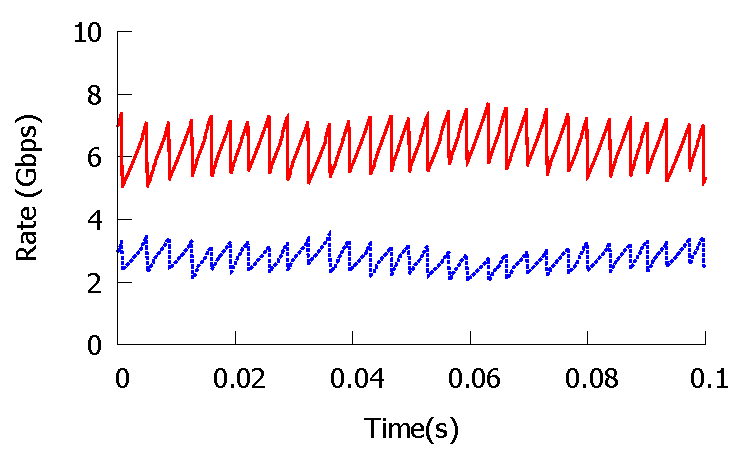
\includegraphics[width=0.3\textwidth]{figures/timely_stability_2f73.pdf}
\label{fig:ts2f73}
}
\vspace{-0.5em}
\caption{Performance of two TIMELY flows under different starting conditions}
\label{fig:timely_unstable}
\vspace{-1em}
\end{figure*}

This is equivalent to changing the $\le$ sign on line 9 of
Algorithm~\ref{fig:timely_algo} to $<$. This makes little difference in
practice, since floating point computations for $g_i$ rarely yield an exact zero
value -- we have verified this via simulations. With this modification, we can
obtain the condition that with $g_i =0$, $\tfrac{dq}{dt} = 0$, $\tfrac{dg_i}{dt} =
0$ and $C*T_{low} < q < C*T_{high}$. However, now we run into the issue that
TIMELY moves from zero fixed points to \emph{infinite} fixed points!

\begin{thm}[Infinite fixed points]
The system described by Figure~(\ref{fig:timely_model}), with
modification introduced in Equation~\ref{eq:timely_r_modified} has
infinite fixed points
\end{thm}
\begin{proof}
To obtain ${dg_i}/{dt} =0$, we need $g_i = 0$ and ${dq}/{dt} = 0$.  Note that $q$
cannot converge to a value outside of the thresholds $ C*{T_{low}}$ and
$C*{T_{high}}$ as that would imply ${dR_i}/{dt} \ne 0$.

Any value of $q$ such that $C*T_{low} < q < C*T_{high}$ makes ${dR_i}/{dt} = 0$
for any value of $R_i$ as long as $\sum_{i} R_i(t) =  C$ and hence $q$
and $R_i$ have
infinitely many fixed points. 
\end{proof}

There is no requirement that at the fixed point $R_i = {C}/{N}$. In fact,
${R_{i}}/{R_{j}}, i \ne j$ is not even bounded, so we cannot make any
claims on the fairness of TIMELY. Thus the fixed point of TIMELY is entirely
unpredictable. This is borne out by the simulation results shown in
Figure~\ref{fig:timely_unstable}, where we only change the start time and
initial rates of two flows, keeping everything else constant, and we end up in
completely different operating regimes.

\para{Impact of per-burst pacing:}
This analysis begs the question -- why does TIMELY work well in practice, as
reported in~\cite{timely}? The answer appears to lie in the fact that the TIMELY
implementation does not use hardware rate limiters.  Instead, the TIMELY
implementation controls rate by adjusting delay between successive transmissions
of chunks that can be as large as 64KB. Each chunk is sent out at or near line rate.

The results shown in Figure~\ref{fig:timely_unstable} were obtained with
per-packet pacing. If, instead we user per-burst pacing, TIMELY appears to
converge, as shown in Figure~\ref{fig:timely_burst_73_16}. The bursts introduce
enough ``noise'' to de-correlate the flows, and this appears to lead the system
to a relatively stable fixed point. We attempted to mathematically prove that
per-burst pacing would lead to a unique fixed point, but were unable to do so.

In any case, per-burst pacing is not ideal, since it can lead to large
oscillations in queue length, leading to poor utilization. This is apparent in
Figure~\ref{fig:timely_burst_55_64}, where we use 64KB chunks. The initial
chunks sent by the two senders arrive at the switch near-simultaneously (i.e.
``incast''), and both flows receive a very large RTT sample. This causes TIMELY
to reduce its rate drastically (line 8 in the TIMELY algorithm). Since the
subsequent rate increase occurs in small steps ($\delta = 10Mbps$, see line
6.)\footnote{HAI kicks in only after $RTT > T_{low}$. See Algorithm 1 in \cite{timely}}, it takes a long time for the flow rates to climb back to their fair
share. 

These problems can be mitigated to some extent by sending bursts at less than
line rate\footnote{Indeed, the TIMELY does this, see \S~5
in~\cite{timely}.}, by adjusting the burst size, or by adjusting the $T_{min}$
threshold. However, such tuning is fragile, since the right values of these
parameters depend not just on the link speed, but also on the number of
competing flows, which is unknown at the time of configuration. 

In summary, while burst pacing can lead to a fixed point by introducing noise,
it can lead to other problems. Rather than rely on ``noise'' to ensure
convergence and stability, we propose a simple fix to the TIMELY algorithm.

\begin{figure*}[t]
\centering
\mbox{
\begin{minipage}{0.62\textwidth}
\subfigure[Two flows starting at 7 and 3Gbps, 16KB burst] { 
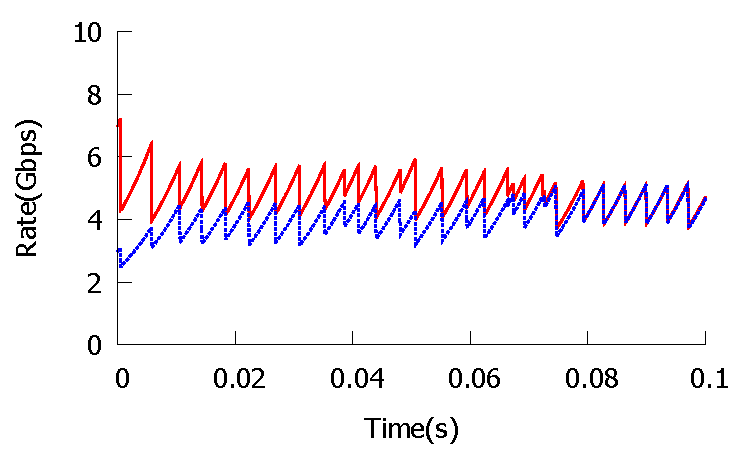
\includegraphics[width=0.47\textwidth]{figures/2f73burst16.pdf}
\label{fig:timely_burst_73_16}
}
\subfigure[Two flows starting at 5Gbps, 64KB burst] { 
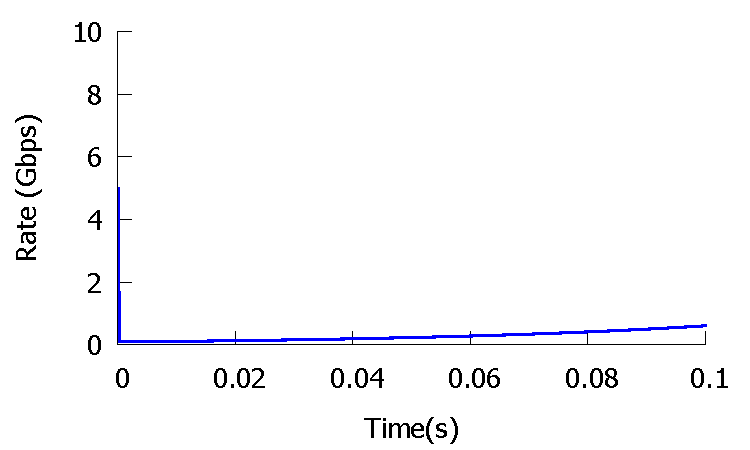
\includegraphics[width=0.47\textwidth]{figures/timely_bursty_64_rate.pdf}
\label{fig:timely_burst_55_64}
}
\vspace{-1em}
\caption{TIMELY with bursts}
\label{fig:timely_sim_bursty}
\end{minipage}
\begin{minipage}{0.36\textwidth}
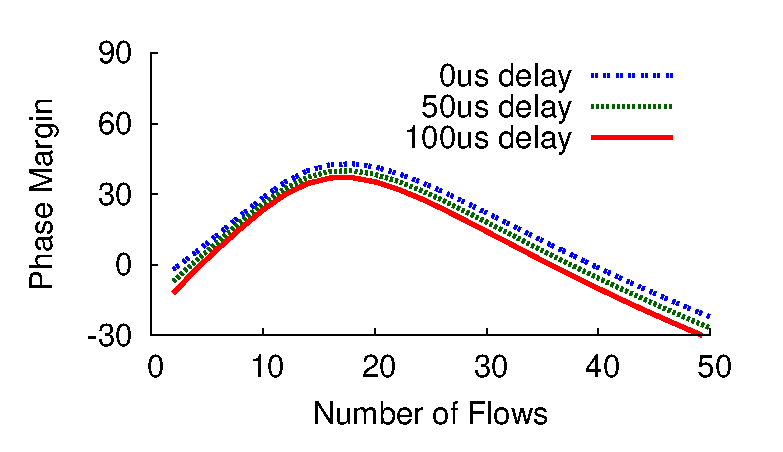
\includegraphics[width=0.99\textwidth]{figures/timely_stability.eps}
\caption{Patched TIMELY stability}
\label{fig:timely_stability}
\end{minipage}
}
\end{figure*}
